%% LyX 1.1 created this file.  For more info, see http://www.lyx.org/.
%% Do not edit unless you really know what you are doing.
\documentclass[english]{article}
\usepackage{helvet}
\usepackage[T1]{fontenc}
\usepackage[latin1]{inputenc}
% \usepackage{babel}
\usepackage{graphics}

\makeatletter

%%%%%%%%%%%%%%%%%%%%%%%%%%%%%% LyX specific LaTeX commands.
\providecommand{\LyX}{L\kern-.1667em\lower.25em\hbox{Y}\kern-.125emX\@}

%%%%%%%%%%%%%%%%%%%%%%%%%%%%%% Textclass specific LaTeX commands.
 \newenvironment{lyxcode}
   {\begin{list}{}{
     \setlength{\rightmargin}{\leftmargin}
     \raggedright
     \setlength{\itemsep}{0pt}
     \setlength{\parsep}{0pt}
     \normalfont\ttfamily}%
    \item[]}
   {\end{list}}
 \usepackage{verbatim}

%%%%%%%%%%%%%%%%%%%%%%%%%%%%%% User specified LaTeX commands.
\usepackage{dsfont}

% No date please
\date{}
\fontfamily{cmss}
\selectfont
\makeatother
\begin{document}
% This is for \LyX


\newcommand{\bfrac}[2]{\frac{#1 }{#2 }}



\newcommand{\nth}{^{\textrm{th}}}



\newcommand{\R}{R}



\newcommand{\N}{N}



\newcommand{\Z}{Z}



\newcommand{\tra}{^{T}}



\newcommand{\xx}{\mathbf{x}}


% This is for \LaTeX

\fontfamily{cmss}\selectfont

\renewcommand{\R}{{\mathds{R}}} 

\renewcommand{\N}{{\mathds{N}}}

\renewcommand{\Z}{{\mathds{Z}}}

\renewcommand{\tra}{^{\top}}

\renewcommand{\bfrac}[2]{\frac{{\textstyle #1 }}{{\textstyle #2 }}}


\title{Mini-HOWTO on using Octave for Unconstrained Nonlinear Optimization%
\thanks{Author : Etienne Grossmann \texttt{<etienne@egdn.net>} (soon
replaced by {}``Octave-Forge developers''?). This document is free
documentation; you can redistribute it and/or modify it under the
terms of the GNU Free Documentation License as published by the Free
Software Foundation.\protect \\
.~~~This is distributed in the hope that it will be useful, but
WITHOUT ANY WARRANTY; without even the implied warranty of MERCHANTABILITY
or FITNESS FOR A PARTICULAR PURPOSE.
}}

\maketitle
\begin{comment}
Keywords: nonlinear optimization, octave, tutorial, Nelder-Mead, Conjugate
Gradient, Levenberg-Marquardt
\end{comment}
Nonlinear optimization problems are very common and when a solution
cannot be found analytically, one usually tries to find it numerically.
This document shows how to perform unconstrained nonlinear minimization
using the Octave language for numerical computation. We assume to
be so lucky as to have an initial guess from which to start an iterative
method, and so impatient as to avoid as much as possible going into
the details of the algorithm. In the following examples, we consider
multivariable problems, but the single variable case is solved in
exactly the same way.

All the algorithms used below return numerical approximations of \emph{local
minima} of the optimized function. In the following examples, we minimize
a function with a single minimum (Figure~\ref{fig:function}), which
is relatively easily found. In practice, success of optimization algorithms
greatly depend on the optimized function and on the starting point.


\section*{\fontfamily{cmss} \selectfont A simple example}


\begin{figure}
{\centering \raisebox{6mm}{\resizebox*{0.3\textwidth}{!}{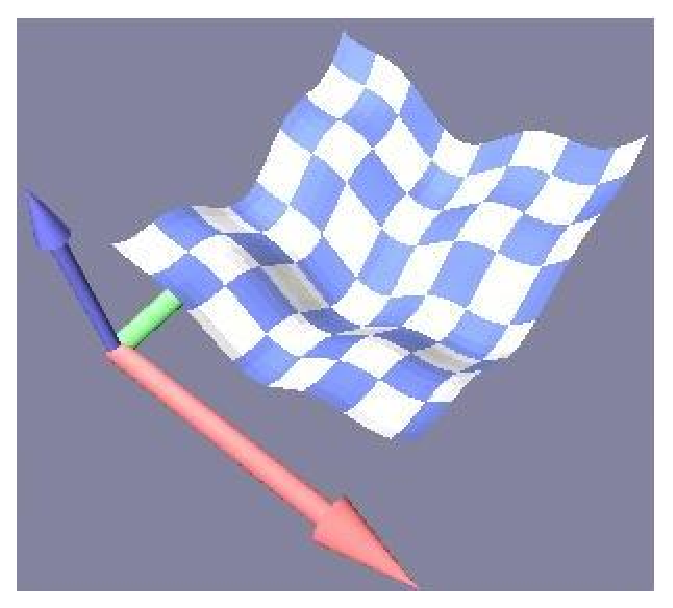
\includegraphics{figures/2D_slice-3.eps2}} }~\resizebox*{0.5\textwidth}{!}{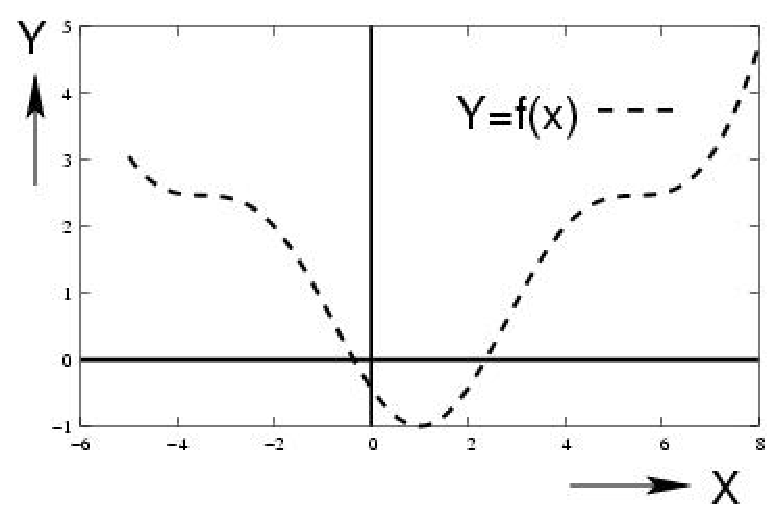
\includegraphics{figures/optim_tutorial_slice.eps}} \par}


\caption{\label{fig:function} 2D and 1D slices of the function that is minimized
throughout this tutorial. Although not obvious at first sight, it
has a unique minimum.}
\end{figure}


We will use a call of the type

\begin{lyxcode}
{[}x\_best,~best\_value,~niter{]}~=~minimize~(func,~x\_init)
\end{lyxcode}
to find the minimum of \[
\begin{array}{cccc}
f\, : & \left( x_{1},.x_{2},x_{3}\right) \in \R ^{3} & \longrightarrow  & \left( x_{1}-1\right) ^{2}/9+\left( x_{3}-1\right) ^{2}/9+\left( x_{3}-1\right) ^{2}/9\\
 &  &  & -\cos \left( x_{1}-1\right) -\cos \left( x_{2}-1\right) -\cos \left( x_{3}-1\right) .
\end{array}\]


The following commands should find a local minimum of \( f() \),
using the Nelder-Mead (aka {}``downhill simplex'') algorithm and
starting from a randomly chosen point \texttt{x0}~:

\begin{lyxcode}
function~cost~=~foo~(xx)

~~xx-{}-;~~

~~cost~=~sum~(-cos(xx)+xx.\textasciicircum{}2/9);

endfunction

x0~=~{[}-1,~3,~-2{]};

{[}x,v,n{]}~=~minimize~(\char`\"{}foo\char`\"{},~x0)
\end{lyxcode}
The output should look like~:

\begin{lyxcode}
x~=

~~1.00000~1.00000~1.00000



v~=~-3.0000

n~=~248
\end{lyxcode}
This means that a minimum has been found in \( \left( 1,1,1\right)  \)
and that the value at that point is \( -3 \). This is correct, since
all the points of the form \( x_{1}=1+2i\pi ,\, x_{2}=1+2j\pi ,\, x_{3}=1+2k\pi  \),
for some \( i,j,k\in \N  \), minimize \( f() \). The number of function
evaluations, 248, is also returned. Note that this number depends
on the starting point. You will most likely obtain different numbers
if you change \texttt{x0}.

The Nelder-Mead algorithm is quite robust, but unfortunately it is
not very efficient. For high-dimensional problems, its execution time
may become prohibitive.


\section*{\fontfamily{cmss} \selectfont Using the first differential}

Fortunately, when a function, like \( f() \) above, is differentiable,
more efficient optimization algorithms can be used. If \texttt{minimize()}
is given the differential of the optimized function, using the \texttt{\char`\"{}df\char`\"{}}
option, it will use a conjugate gradient method.

\begin{lyxcode}
\#\#~Function~returning~partial~derivatives

function~dc~=~diffoo~(x)

~~~~x~=~x(:)'~-~1;

~~~~dc~=~sin~(x)~+~2{*}x/9;

endfunction

{[}x,~v,~n{]}~=~minimize~(\char`\"{}foo\char`\"{},~x0,~\char`\"{}df\char`\"{},~\char`\"{}diffoo\char`\"{})
\end{lyxcode}
This produces the output~:

\begin{lyxcode}
x~=

~~1.00000~1.00000~1.00000

v~=~-3~

n~=

~~108~6
\end{lyxcode}
The same minimum has been found, but only 108 function evaluations
were needed, together with 6 evaluations of the differential. Here,
\texttt{diffoo()} takes the same argument as \texttt{foo()} and returns
the partial derivatives of \( f() \) with respect to the corresponding
variables. It doesn't matter if it returns a row or column vector
or a matrix, as long as the \( i\nth  \) element of \texttt{diffoo(x)}
is the partial derivative of \( f() \) with respect to \( x_{i} \)
.


\section*{\fontfamily{cmss} \selectfont Using numerical approximations of
the first differential}

Sometimes, the minimized function is differentiable, but actually
writing down its differential is more work than one would like. Numerical
differentiation offers a solution which is less efficient in terms
of computation cost, but easy to implement. The \texttt{\char`\"{}ndiff\char`\"{}}
option of \texttt{minimize()} uses numerical differentiation to execute
exactly the same algorithm as in the previous example. However, because
numerical approximation of the differentia is used, the outpud may
differ slightly~:

\begin{lyxcode}
{[}x,~v,~n{]}~=~minimize~(\char`\"{}foo\char`\"{},~x0,~\char`\"{}ndiff\char`\"{})
\end{lyxcode}
wich yields~:

\begin{lyxcode}
x~=

~~1.00000~1.00000~1.00000

v~=~-3~

n~=

~~78~6
\end{lyxcode}
Note that each time the differential is numerically approximated,
\texttt{foo()} is called 6 times (twice per input element), so that
\texttt{foo()} is evaluated a total of (78+6{*}6=) 114 times in this
example.


\section*{\fontfamily{cmss} \selectfont Using the first and second differentials}

When the function is twice differentiable and one knows how to compute
its first and second differentials, still more efficient algorithms
can be used (in our case, a variant of Levenberg-Marquardt). The option
\texttt{\char`\"{}d2f\char`\"{}} allows to specify a function that
returns the value of the function, the first and second differentials
of the minimized function. Entering the commands~: 

\begin{lyxcode}
function~{[}c,~dc,~d2c{]}~=~d2foo~(x)

~~~~c~=~foo(x);

~~~~dc~=~diffoo(x);

~~~~d2c~=~diag~(cos~(x(:)-1)~+~2/9);

end

{[}x,v,n{]}~=~minimize~(\char`\"{}foo\char`\"{},~x0,~\char`\"{}d2f\char`\"{},~\char`\"{}d2foo\char`\"{})~
\end{lyxcode}
produces the output~:

\begin{lyxcode}
x~=

~~1.0000~1.0000~1.0000

v~=~-3

n~=

~~34~5
\end{lyxcode}
This time, 34 function evaluations, and 5 evaluations of \texttt{d2foo()}
were needed.


\section*{\fontfamily{cmss} \selectfont Summary}

We have just seen the most basic ways of solving nonlinear unconstrained
optimization problems. The online help system of Octave (try e.g.
{}``\texttt{help minimize}'') will yield information on other issues,
such as \emph{passing extra arguments} to the minimized function,
\emph{controling the termination} of the optimization process, choosing
the algorithm etc.

\begin{lyxcode}
\end{lyxcode}

\end{document}
